\documentclass[11pt]{article}
\usepackage{graphicx}
\usepackage{wrapfig}

\title{Modivation}
\author{Karl Menzel}

\begin{document}

\maketitle

\section{Modivation}
\indent Animals of some species tend to not be randomly distributed throughout space, instead animals tend to be group up into populations and sub populational groups including social groups.  Understanding these social groups can be important for understanding things such as the distribution of disease within the population \cite{weber-2013}.  Computational methods using graphs methods have proven to be useful when identifying and social groups and subgroups in highly dynamic free ranging systems \cite{Ramos-Fernandez-2009,marsh-2011}.  These clustering studies have used weighted graphs created by some measure of association whether by observational studies or by radio collars. Weber et. al. (2013) does not implement clustering on their badger social network, but they use measures of inbetweennes which are used on some clustering methods.
\begin{wrapfigure}{h}{0.4\textwidth}
%\centering % center the figure
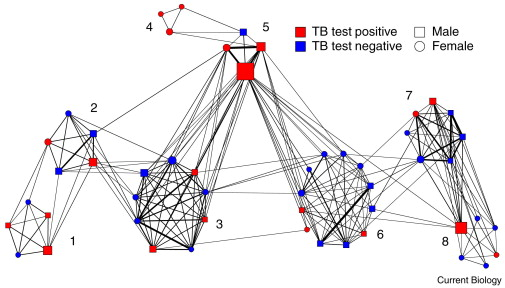
\includegraphics[width=\linewidth]{weberImage.jpg}
\caption{Figure form weber et. al. (2013) ilistrating the social interactions of badgers and distrobution of TB} % caption
\label{badger} % add a label to reference it
\end{wrapfigure}   Understanding the relationship between the clustering of these badgers and inbetweennes will shed some light on the relationships of the badgers. 

\indent I plan to use the badger social network data that we used for our first lab and homework assignment.  My overall goals for the project are to recreate the figure found in Weber et. al. (2013) and apply clustering methods to the data to understand their effectiveness and relationships of betweennes.  The figure in Weber et. al. (2013) includes results or TB test, edge betweenness centrality, and among group flow-betweenness which is a measure of how much the individual or interaction allow for transfer of information in the network.  For my project, I will focus on edge betweennes centrality.  For clustering, cluster with the raw interaction data.  I anticipate implementing the edge betweenness centrality to be the hardest part of the project.  I have found the paper where it is described in but it is a new algorithm that that I am not familiar with and we have not talked about it in class.




This is the paper that desribes the measure of centrality \cite{freeman-1991}.  Main paper is \cite{weber-2013}

\bibliographystyle{plain}
\bibliography{badger}  %% this is test.bib file.

\end{document}

